%%%%%%%%%%%%%%%%%%%%%%%%%%%%%%%%%%%%%%%%%%%%%%%%%%%%%%%
% \documentclass{article}
% \documentclass[12pt]{article}
\documentclass[twocolumn]{article}
% Dùng để thêm hình ảnh
\usepackage{graphicx}
% Dùng để di chuyển các tham chiếu
\usepackage{hyperref}
% Dùng để tạo văn bản ngẫu nhiên
\usepackage{lipsum}
% Dùng để cố định hình ảnh \begin{figure}[H]
\usepackage{float}
% Dùng để tài liệu tham khảo
\usepackage{cite}
% 
\usepackage{tikz}
% 
% Dùng để sử dụng màu
\usepackage{xcolor}
% \pagecolor[RGB]{40, 42, 54} % Đặt màu nền
% \color[RGB]{18, 161, 24} % Đặt màu chữ
% 
\usepackage{fancyhdr}







% Dùng để tạo keywords
\providecommand{\keywords}[1]{\textbf{\textit{Keywords.}} #1}


% 
\definecolor{myblack}{RGB}{0,0,0}
\newcommand{\myrect}{\tikz[baseline=(char.base)]{\node[anchor=text, rectangle, inner sep=5pt, fill=myblack, text=white] (char) {\normalfont\small SURVEY PAPER};}}

% Redefine \maketitle to disable page numbering
\let\oldmaketitle\maketitle
\renewcommand{\maketitle}{
  \thispagestyle{empty}
  \oldmaketitle
}
%%%%%%%%%%%%%%%%%%%%%%%%%%%%%%%%%%%%%%%%%%%%%%%%%%%%%%%

 
 


 


\pagestyle{fancy}
\fancyhf{}
% \renewcommand{\headrulewidth}{0pt} % Loại bỏ đường gạch ngang
\lhead{\raisebox{-0.4\height}{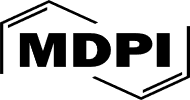
\includegraphics[width=2cm]{pictures/MDPI.png}}}
\rhead{\myrect}




% Thiết lập chân trang
% \fancyfoot[L]{Copyright \textcopyright \the\year. Faculty of Applied Mathematics and Informatics}
\fancyfoot[C]{\thepage} % Chân trang phải
% \fancyfoot[R]{\thepage} % Chân trang phải

% Thêm thanh ngang phía dưới chân trang
\renewcommand{\footrulewidth}{0.4pt}
\renewcommand{\footruleskip}{0mm}
\renewcommand{\footrule}{\hbox to\headwidth{\color{black}\leaders\hrule height \footrulewidth\hfill}}
  
%%%%%%%%%%%%%%%%%%%%%%%%%%%%%%%%%%%%%%%%%%%%%%%%%%%%%%%
\begin{document}
%%%%%%%%%%%%%%%%%%%%%%%%%%%%%%%%%%%%%%%%%%%%%%%%%%%%%%%
% Tiêu đề
\title{A Survey of Security and Privacy Challenges in Cloud Computing and Desirable Solutions In Future}
% Tác giả
\author{
Mai Thanh Duy 20227225 \\
Tran Duc Toan 20195929 \\
Vu Van Nghia 20206205
}
\maketitle
%%%%%%%%%%%%%%%%%%%%%%%%%%%%%%%%%%%%%%%%%%%%%%%%%%%%%%%
\begin{abstract}
    As organizations increasingly transition critical operations to the cloud, ensuring strong security measures becomes paramount. However, the evolving threat landscape poses significant challenges as cyber adversaries continually devise sophisticated tactics to exploit vulnerabilities in cloud infrastructure. This article gives an overview of cloud computing infrastructure, how cloud computing works, as well as how major companies around the world implement cloud computing transformation. The article also provides in-depth analysis of the current threats facing cloud security, from data breaches and insider threats to sophisticated attacks and vulnerabilities in the supply chain. By examining real-world case studies and industry reports, we identify key vulnerabilities that leave cloud environments at risk of exploitation. Furthermore, this article includes the security options offered by the major vendors, thereby exploring the emerging trends and technologies that are shaping the future of cloud security. Additionally, we discuss the role of automation, orchestration, and artificial intelligence in enhancing threat detection and response in the cloud. By fostering collaboration among industry stakeholders and leveraging innovative approaches, organizations can proactively mitigate risk and build resilient cloud architectures to the challenges of the future threat landscape.
\end{abstract}

\keywords{xxx, xxx, yyy, xxx, xxx, xxx, yyy}

\section{INTRODUCTION}
In recent years, cloud computing has emerged as a dominant paradigm in the realm of IT infrastructure, driven by a confluence of market forces and technological advancements. The dynamic nature of modern business environments has propelled organizations towards adopting cloud-based solutions to meet their evolving computational needs. With an ever-expanding array of enterprise services and applications, companies are increasingly reliant on cloud infrastructures to support their operations.

% …………………………………………………………………………………………………………
% (chưa biết thêm thông tin gì vào)
% …………………………………………………………………………………………………………………

xxxxxxxxxxxxxxxxxxxxx

xxxxxxxxxxxxxxxxxxxxx

xxxxxxxxxxxxxxxxxxxxx

xxxxxxxxxxxxxxxxxxxxx

This article explores the multifaceted landscape of cloud security, divided into five chapters. In Security Issues and Threats: Delving into the various security concerns that plague cloud environments, this chapter examines real-world examples and their implications for cloud security. In Attack Patterns: Understanding the methods and patterns used by attackers is crucial for devising effective security measures. This chapter explores common attack vectors targeting cloud infrastructures, providing insights into malicious strategies. In Current Techniques to Counter: To mitigate the risks posed by security threats, organizations deploy a range of techniques and technologies. This chapter reviews the current state-of-the-art approaches for securing cloud environments. Finally, in Future Directions: Looking ahead, the landscape of cloud security is poised for continued evolution. This final chapter examines emerging trends and technologies that are shaping the future of cloud security

% \section{METHODS}
% \lipsum[1]

% \section{RESULTS}
% \lipsum[1]

% \section{DISCUSSION}
% \lipsum[1]

% \section{CONCLUSION}
% \lipsum[1]

%%%%%%%%%%%%%%%%%%%%%%%%%%%%%%%%%%%%%%%%%%%%%%%%%%%%%%%
\renewcommand{\refname}{REFERENCES}
\bibliographystyle{plain}
\bibliography{References}
%%%%%%%%%%%%%%%%%%%%%%%%%%%%%%%%%%%%%%%%%%%%%%%%%%%%%%%
\newpage
\section{EXAMPLE \LaTeX}
% Trang mới
\newpage

% Văn bản ngẫu nhiên
\lipsum[1]

% Thêm hình ảnh
\begin{figure}[H]
\centering

\includegraphics[scale = 0.4]{pictures/HUST.png}
\caption{xxx}
\end{figure}

% Thêm hình bảng

% Dùng tham khảo
References \cite{syropoulos2007digital}
%%%%%%%%%%%%%%%%%%%%%%%%%%%%%%%%%%%%%%%%%%%%%%%%%%%%%%%
\end{document} % Kết thúc
%%%%%%%%%%%%%%%%%%%%%%%%%%%%%%%%%%%%%%%%%%%%%%%%%%%%%%%


   
